% the introduction section...

\chapter{مقدمه} \label{chapter:introduction}

\paragraph*{}

\section{موزه تاریخ طبیعی}
اولين موزه تاريخ طبيعي در قرن
هفدهم و در شهر پاريس افتتاح شد.
در ابتدا عموم مردم اجازه بازديد از اينگونه موزه‌ها را نداشتند زيرا يا به
صورت مجموعه هاي خصوصي و يا زير نظر متخصصان علوم طبيعي قرار داشتند. اما به تدريج درهاي آن به
روي مردم باز شد.

وظيفه اصلي موزه هاي تاريخ طبيعي آشنايي جامعه و ارتقاء آگاهي هاي عمومي در مورد جانوران ، گياهان و 
ساير موجودات زنده ، فسيل ها ، سنگ ها ، كاني ها و همچنين زيستگاه هاي طبيعي است . اين مكان ها 
عامل انتقال وتوسعه دانش ودرك دنياي طبيعي وجايگاه ونقش انسان درآن مي باشند . موزه هاي تاريخ طبيعي
از طريق نمايشگاهها وبرنامه هاي آموزشي كه با اهداف خاص تدوين مي شوند به تفسير وشرح جايگاه واجزاء
طبيعت ،ارتباط آنها با يكديگر وبا انسان،اهميت حفظ آن واهميت ايجادارتباط بين طبيعت وانسان مي
پردازند.آنها درك انسان را از محيط اطراف خود افزايش مي دهندوفرصتهايي براي كسب دانش وغني ساختن
فرهنگ فراهم مي آورند.

موزه هاي تاريخ طبيعي ميتوانند از طريق نمايشگاهها و فعاليت هاي آموزشي واطلاعات
نهفته درمجموعه ها ودرواقع كارشناسان خود دانش لازم را به مردم عادي انتقال دهند.موزه هاي امروزي مي
توانند طرز تفكر مردم را درمورد طبيعت تغيير دهند ورفتار وديدگاههاي مثبتي را نسبت به محيط طبيعي
ترويج نمايند چرا كه بهتر زيستن نياز به دانش زيست محيطي وآموزش دارد وآغاز هر حياتي مستلزم اهميت
دادن به حيات وحش ،آب وخاك ومنابع طبيعي است . در عين حال بخش هاي علمي و بايگاني موزه هاي تاريخ
طبيعي داراي مجموعه هاي وسيعي از جانوران ، گياهان ، فسيل ها ، سنگ ها و كاني ها است كه مي توانند مواد
و اطلاعات لازم را جهت تحقيق زيست شناسان و دانشجويان علوم طبيعي فراهم آورند.


\newpage

گروه موزه تاریخ طبیعی و دخایر ژنتیکی شامل:
\begin{itemize}
    \item موزه تنوع زیستی
    \item کارگاه تاکسیدرمی
    \item بخش‌های ستادی
\end{itemize}
است.

وظایف این گروه عبارتند از:

\begin{itemize}
    \item ارتقاء ارتباط و سطح آگاهي هاي زيست محيطي اقشار مختلف جامعه از طريق نمايشگاه
    هاي تاريخ طبيعي مركز و ادارات كل كشور
    \item نظارت بر فعاليت هاي موزه‌هاي ادارات كل
    \item ايجاد ارتباطات بين المللي و به روز رساني سطح اطلاعات دفتر
    \item آماده سازي نمونه‌ها در كارگاه تاكسيدرمي
    \item تهيه دستور العمل‌هاي مورد نياز و نظارت و اظهار نظر در ارتباط با ايجاد موزه هاي تاريخ
    طبيعي و همچنين كارگاه هاي تاكسيدرمي در كشور
\end{itemize}

\section{موزه تنوع زيستي}
موزه تنوع زيستي ايران در فضاي داخلي بالغ بر 1400 متر مربع در مجموعه علمي ،پژوهشي و تفرجگاهي
پرديسان قرار گرفته است و زير نظر سازمان حفاظت محيط زيست مي باشد. 
ساختمان موزه درراستاي ايجاد محيط علمي، پژوهشي و همگام با سياست هاي سازمان حفاظت محـيط زيسـت
بنا نهاده شده است. اين مجموعه كه بصورت نمايشگاه تخصصي گونه هاي گياهي ،جانوري و نمونه هاي سـنگ و
كاني و فسيل مي باشد، درفروردين 1383 با حضوررياسـت جمهـوري وقـت و رياسـت قبلـي و فعلـي سـازمان
حفاظت محيط زيست، سركارخانم دكتر ابتكار افتتاح گرديد. اكثريت قريب به اتفاق نمونه هـا واقعـي بـوده و بـا
استفاده از هنر تاكسيدرمي (پوست آرايي) كه در واقع كشيدن پوست حيوان بر روي قالـب مـي باشـد، تهيـه
گرديده است . علاوه بر آن با ايجاد سايت موزه مجازي امكان آشنايي بيننـدگان را از طريـق شـبكه اينترنـت در
ايران و سراسر جهان فراهم نموده است.

\begin{figure}
    \label{fig2.1}
    \centering
    \caption{موقعیت موزه تنوع زیستی روی نقشه}
    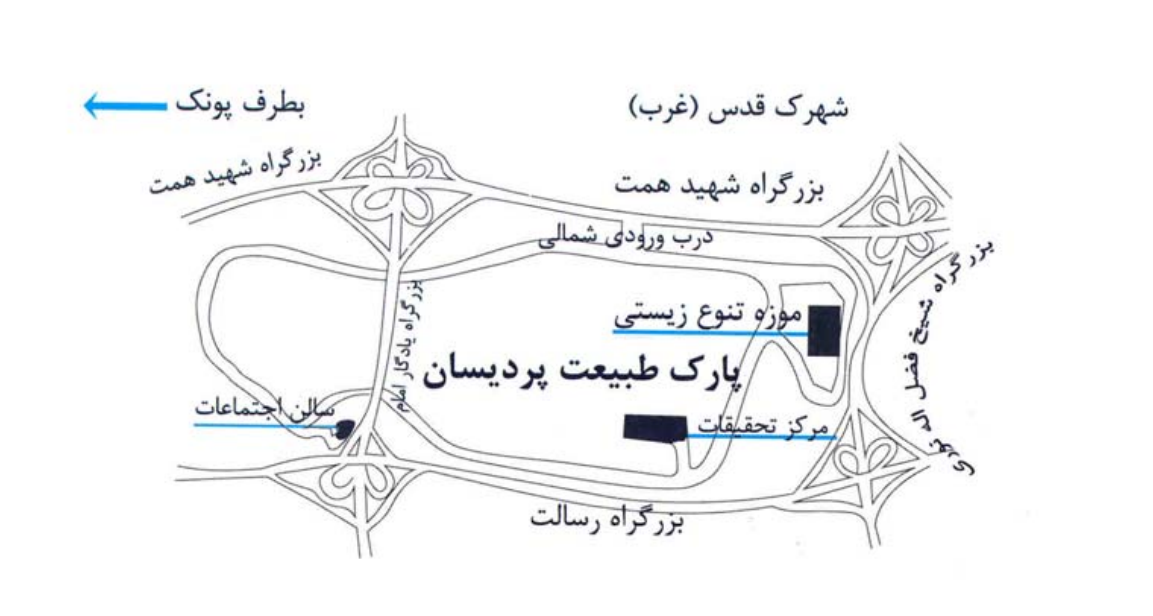
\includegraphics[scale = 0.5]{images/map.PNG}
\end{figure}

بطور كلي سازمان آموزش و پرورش استان تهران با هماهنگي مديريت موزه اقدام به بازديدهاي گروهي دانش
آموزان بالاخص در مقاطع ابتدايي و راهنمايي مي نمايد . علاوه بر اين نظر به قرار گرفتن اين موزه در پارك
طبيعت پرديسان ، افرادي كه به قصد تفرج و گذران اوقات فراغت خود به اين مكان مي آيند قادر به بازديد از
اين موزه مي باشند ، همجنين هنرمندان ، مخصوصا نقاشان كه علاقمند به طراحي از طبيعت و جانوران
هستند از اين نمايشگاه استفاده مي نمايند . فضاي داخلي غرفه هاي موزه تنوع زيستي با الهام از طبيعت ايران
،جهان و زيستگاههاي طبيعي جانوران طراحي و فضاسازي شده است

در موزه تنوع زيستي تقسيم بندي بر اساس سيستم قاره اي – زيسـتگاهي بـوده كـه نمونـه هـاي متعـددي در
زيستگاه هاي مربوطه عرضه شده اند و شامل غرفه هاي ذيل مي باشد:

\begin{itemize}
    \item غرفه نمونه‌های منقرض شده ايران: شامل مجسمه ها ي شير ايراني و ببر خزري
    \item غرفه نمونه هاي كمياب ايران
    \item غرفه تنوع زيستي ايران
    \item غرفه تنوع زيستي جهان
    \item غرفه خليج فارس
    \item غرفه تونل زير دريايي خليج فارس
    \item غرفه درياي مازندران
    \item غرفه قاره آسيا
    \item غرفه قاره اروپا
    \item غرفه قاره آفريقا
    \item غرفه قاره آمريكا
    \item غرفه قاره اقيانوسيه
    \item غرفه زيستگاه قطب جنوب
    \item قاب پوست ببر خزري: اين پوست متعلق به ببر خزري است كه در پارك ملي گلستان به سال 1329شكار شده است.
    \item قاب پروانه ها
    \item ويترين حشرات
    \item اسكلت فيل آسيايي
    \item ويترين سنگ و كانيهاي ايران
    \item ويترين نرمتنان
    \item ويترين فسيلهاي گياهي
    \item ويترين فسيلهاي بي مهرگان
    \item ويترين فسيلهاي ماهيان آب شيرين
    \item تابلوي بازسازي فسيل‌هاي مراغه
    \item ويترين فسيلهاي مهره داران مراغه
\end{itemize}


\begin{figure}
    \label{fig2.2}
    \centering
    \caption{دیورامای نمونه‌‌های منقرض شده}
    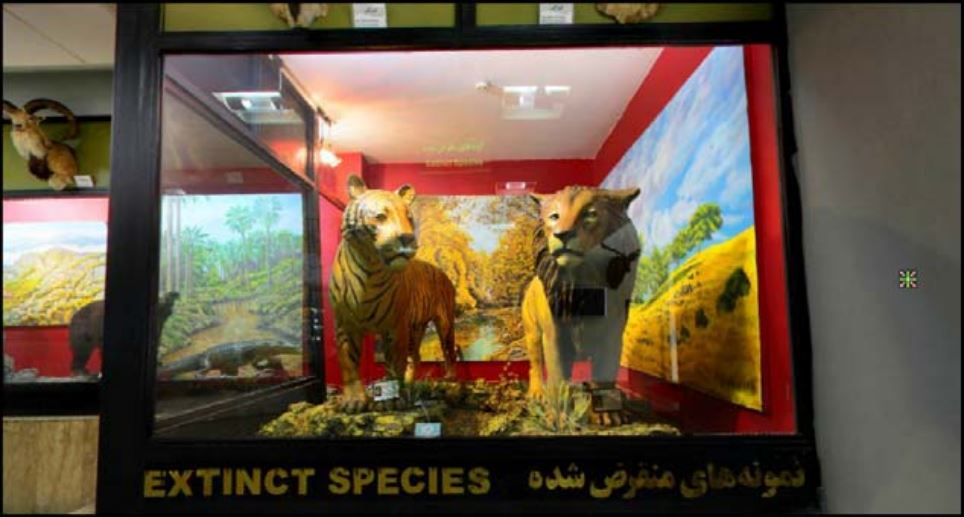
\includegraphics[scale = 0.5]{images/monqarez.jpg}
\end{figure}

